\documentclass[11pt]{article}
\usepackage{amsmath, amssymb, physics, mathtools, bm}
\usepackage{tikz, pgfplots}
\pgfplotsset{compat=1.18}
\usepackage[margin=2.3cm]{geometry}
\usepackage{siunitx, booktabs, hyperref}
\newcommand{\D}{\mathrm{D}}
\newcommand{\de}{\mathrm{d}}
\newcommand{\pd}[2]{\frac{\partial #1}{\partial #2}}
\newcommand{\pdd}[2]{\frac{\partial^{2} #1}{\partial #2^{2}}}
\newcommand{\Lap}{\nabla^{2}}
\title{B1 Flows, Fluctuations and Complexity, 2019 --- Model Solutions}
\author{}
\date{}
\begin{document}
\maketitle

%==============================================================
\section*{Question 1 --- Vorticity, circulation and Couette flow}

\textbf{Problem.} Define vorticity and circulation; treat solid-body rotation and the line vortex; derive the tangential Couette flow between two rotating cylinders, its vorticity and pressure; discuss the Reynolds number and evaluate numerically.

\subsection*{(a) Vorticity and circulation}

Vorticity:
\[ \bm\omega = \nabla\times\vb u. \]
Physical meaning: $\bm\omega$ is twice the local angular velocity of a fluid element; it measures local spin.

Circulation around a closed contour $C$ bounding surface $S$:
\[ \Gamma = \oint_C \vb u\cdot\de\bm\ell = \int_S \bm\omega\cdot\de\vb S. \]
The first form is the line integral of velocity along $C$; the second (Stokes) is the flux of vorticity through any surface spanning $C$.

\subsection*{(b) Solid-body rotation and line vortex}

\textbf{(i)} For solid-body rotation, $\vb u = \bm\Omega\times\vb r$. Take a circle of radius $r$ centred on the axis. Tangential velocity:
\[ u_\theta = \Omega r. \]
Line-integral form of circulation:
\[ \Gamma = \oint_C \vb u\cdot\de\bm\ell = \oint u_\theta\,r\,\de\theta. \]
Substitute $u_\theta = \Omega r$:
\[ \Gamma = \int_0^{2\pi}\!(\Omega r)(r)\,\de\theta. \]
Factor out constants:
\[ \Gamma = \Omega r^2\!\int_0^{2\pi}\!\de\theta. \]
Evaluate the integral:
\[ \Gamma = 2\pi\Omega r^2. \]
Apply Stokes with uniform $\omega$ over the enclosed disc:
\[ \Gamma = \int_S \omega\,\de S = \omega\,\pi r^2. \]
Equate the two expressions:
\[ 2\pi\Omega r^2 = \omega\,\pi r^2. \]
Cancel $\pi r^2$:
\[ \omega = 2\Omega. \]
\[ \boxed{\;\bm\omega = 2\bm\Omega.\;} \]

\textbf{(ii)} Line vortex $U_\theta = A/r$, $r>0$. Line-integral circulation on a circle of radius $r$:
\[ \Gamma = \oint U_\theta\,r\,\de\theta. \]
Substitute $U_\theta = A/r$:
\[ \Gamma = \int_0^{2\pi}\!\frac{A}{r}\cdot r\,\de\theta. \]
Cancel the $r$:
\[ \Gamma = A\!\int_0^{2\pi}\!\de\theta. \]
Evaluate:
\[ \Gamma = 2\pi A. \]
Vorticity (axisymmetric):
\[ \omega_z = \frac{1}{r}\dv{r}(rU_\theta). \]
Substitute $rU_\theta = A$:
\[ \omega_z = \frac{1}{r}\dv{r}(A). \]
Derivative of constant vanishes:
\[ \omega_z = 0,\qquad r>0. \]
Comment: vorticity vanishes everywhere except at $r=0$ but $\Gamma\neq 0$, so all the vorticity is concentrated as a delta function on the axis. The flow is irrotational outside the singular core.

\subsection*{(c) Couette flow between rotating cylinders}

Continuity (incompressible, axisymmetric, $U_z=0$):
\[ \frac{1}{r}\pd{(rU_r)}{r} = 0. \]
Integrate and apply $U_r=0$ on the walls:
\[ U_r = 0. \]
Symmetry gives $\partial_\theta(\cdot)=0$ and steady $\partial_t(\cdot)=0$. Navier--Stokes simplifies; radial component (centripetal balance):
\begin{equation}
-\frac{U_\theta^{2}}{r} = -\frac{1}{\rho}\pd{p}{r}.
\label{eq:nsr}
\end{equation}
Tangential component:
\begin{equation}
0 = \nu\!\left[\frac{1}{r}\dv{r}\!\left(r\dv{U_\theta}{r}\right) - \frac{U_\theta}{r^2}\right].
\label{eq:nstheta}
\end{equation}
Rewrite the bracket as a total derivative:
\[ \dv{r}\!\left[\frac{1}{r}\dv{r}(rU_\theta)\right] = 0. \]
Integrate once (call the constant $2C_1$):
\[ \frac{1}{r}\dv{r}(rU_\theta) = 2 C_1. \]
Multiply by $r$:
\[ \dv{r}(rU_\theta) = 2C_1 r. \]
Integrate again:
\[ rU_\theta = C_1 r^2 + C_2. \]
Divide by $r$:
\[ U_\theta(r) = C_1 r + \frac{C_2}{r}. \]
Boundary conditions (no-slip):
\[ U_\theta(r_1) = \Omega_1 r_1,\qquad U_\theta(r_2) = \Omega_2 r_2. \]
Substitute $U_\theta = C_1 r + C_2/r$ at $r=r_1$:
\[ C_1 r_1 + C_2/r_1 = \Omega_1 r_1. \]
Similarly at $r=r_2$:
\[ C_1 r_2 + C_2/r_2 = \Omega_2 r_2. \]
Multiply the first by $r_1$:
\[ C_1 r_1^2 + C_2 = \Omega_1 r_1^2. \]
Multiply the second by $r_2$:
\[ C_1 r_2^2 + C_2 = \Omega_2 r_2^2. \]
Subtract the first equation from the second:
\[ C_1(r_2^2 - r_1^2) = \Omega_2 r_2^2 - \Omega_1 r_1^2. \]
Divide by $r_2^2-r_1^2$:
\[ \boxed{\;C_1 = \frac{\Omega_2 r_2^2 - \Omega_1 r_1^2}{r_2^2 - r_1^2}.\;} \]
Substitute back into $C_1 r_1^2 + C_2 = \Omega_1 r_1^2$:
\[ C_2 = \Omega_1 r_1^2 - C_1 r_1^2. \]
Factor $r_1^2$:
\[ C_2 = r_1^2(\Omega_1 - C_1). \]
Insert $C_1$:
\[ C_2 = r_1^2\!\left[\Omega_1 - \frac{\Omega_2 r_2^2 - \Omega_1 r_1^2}{r_2^2 - r_1^2}\right]. \]
Combine over a common denominator:
\[ C_2 = r_1^2\,\frac{\Omega_1(r_2^2-r_1^2) - \Omega_2 r_2^2 + \Omega_1 r_1^2}{r_2^2-r_1^2}. \]
Simplify the numerator:
\[ C_2 = r_1^2\,\frac{(\Omega_1-\Omega_2)r_2^2}{r_2^2-r_1^2}. \]
Hence
\[ \boxed{\;C_2 = \frac{(\Omega_1-\Omega_2)\,r_1^2 r_2^2}{r_2^2 - r_1^2}.\;} \]
Vorticity (axisymmetric):
\[ \omega_z = \frac{1}{r}\dv{r}(rU_\theta). \]
Substitute $rU_\theta = C_1 r^2 + C_2$:
\[ \omega_z = \frac{1}{r}\dv{r}\!\left(C_1 r^2 + C_2\right). \]
Differentiate:
\[ \omega_z = \frac{1}{r}(2 C_1 r). \]
Cancel $r$:
\[ \omega_z = 2C_1. \]
Physical meaning of $C_1$: the flow consists of a solid-body rotation at angular rate $C_1$ (carrying uniform vorticity $2C_1$) plus an irrotational line-vortex part $C_2/r$.

Pressure: rearrange \eqref{eq:nsr}:
\[ \dv{p}{r} = \frac{\rho\,U_\theta^2}{r}. \]
Square $U_\theta = C_1 r + C_2/r$:
\[ U_\theta^2 = \left(C_1 r + \frac{C_2}{r}\right)^{\!2}. \]
Expand the square:
\[ U_\theta^2 = C_1^2 r^2 + 2 C_1 C_2 + \frac{C_2^2}{r^2}. \]
Divide by $r$:
\[ \frac{U_\theta^2}{r} = C_1^2 r + \frac{2C_1 C_2}{r} + \frac{C_2^2}{r^3}. \]
Integrate term by term:
\[ p(r) = p_0 + \rho\!\left[\int C_1^2 r\,\de r + \int\frac{2C_1 C_2}{r}\,\de r + \int\frac{C_2^2}{r^3}\,\de r\right]. \]
Evaluate the three integrals:
\[ \boxed{\;p(r) = p_0 + \rho\!\left[\tfrac12 C_1^2 r^2 + 2 C_1 C_2 \ln r - \tfrac12\,\frac{C_2^2}{r^2}\right].\;} \]

\subsection*{(d) Reynolds number and numerics}

$Re=\Omega_1 r_1(r_2-r_1)/\nu$ measures inertial : viscous forces, with the gap $r_2-r_1$ as the relevant length and $\Omega_1 r_1$ as the relevant velocity. For $Re<50$ the laminar Couette profile above holds. Increasing $\Omega_1$, $r_2-r_1$, or decreasing $\nu$ raises $Re$; beyond a critical value the flow undergoes Taylor--Couette instability (Taylor vortices) and eventually turbulence.

Data: $r_1 = \SI{0.25}{m}$, gap $d = r_2-r_1 = \SI{5e-3}{m}$, $\mu = \SI{0.02}{Pa\,s}$, $\rho = \SI{900}{kg\,m^{-3}}$.

Convert rpm to rad/s:
\[ \Omega_1 = 20\cdot\frac{2\pi}{60} = \SI{2.094}{rad\,s^{-1}}. \]
Kinematic viscosity:
\[ \nu = \frac{\mu}{\rho} = \frac{0.02}{900} = \SI{2.22e-5}{m^2\,s^{-1}}. \]
Reynolds number formula:
\[ Re = \frac{\Omega_1 r_1(r_2-r_1)}{\nu}. \]
Substitute the values:
\[ Re = \frac{(2.094)(0.25)(5\times 10^{-3})}{2.22\times 10^{-5}}. \]
Multiply numerator:
\[ Re = \frac{2.618\times 10^{-3}}{2.22\times 10^{-5}}. \]
Evaluate:
\[ \boxed{\;Re \approx 118.\;} \]

With $C_2=0$, $U_\theta = C_1 r$ is pure solid-body rotation. From the formula for $C_2$, this requires $\Omega_1=\Omega_2\equiv\Omega$, and then $C_1 = \Omega_1$. Pressure (from boxed result, $C_2=0$):
\[ p(r) - p(r_1) = \tfrac12 \rho C_1^2 (r^2 - r_1^2). \]
Substitute $C_1 = \Omega_1$ and take $r=r_2$:
\[ \Delta p = \tfrac12\rho\Omega_1^2 (r_2^2 - r_1^2). \]
Factor $r_2^2 - r_1^2 = (r_2-r_1)(r_2+r_1)$:
\[ r_2^2 - r_1^2 = (5\times 10^{-3})(0.505). \]
Evaluate:
\[ r_2^2 - r_1^2 = \SI{2.525e-3}{m^2}. \]
Plug in numbers:
\[ \Delta p = \tfrac12 (900)(2.094)^2(2.525\times 10^{-3}). \]
Evaluate the square:
\[ \Delta p = \tfrac12 (900)(4.385)(2.525\times 10^{-3}). \]
Multiply:
\[ \boxed{\;\Delta p \approx \SI{4.98}{Pa}.\;} \]

Interpretation: $Re\approx 118>50$, so the laminar approximation is on the borderline of validity --- Taylor vortices are likely to appear; the calculated $\Delta p$ should therefore be regarded only as the laminar reference value.

%==============================================================
\section*{Question 2 --- Bernoulli, Rayleigh--Plesset and bubble collapse}

\textbf{Problem.} Derive the vorticity form of momentum and the time-dependent Bernoulli equation, then analyse the collapse of a spherical bubble in an incompressible fluid.

\subsection*{(a) Vorticity form of Navier--Stokes}

Navier--Stokes (no gravity, rearranged):
\[ \pd{\vb u}{t} + (\vb u\cdot\nabla)\vb u = -\frac{1}{\rho}\nabla p + \nu\Lap\vb u. \]
Apply the identity $(\vb u\cdot\nabla)\vb u = \nabla(\tfrac12 u^2) + \bm\omega\times\vb u$:
\[ \pd{\vb u}{t} + \nabla\!\left(\tfrac12 u^2\right) + \bm\omega\times\vb u = -\frac{1}{\rho}\nabla p + \nu\Lap\vb u. \]
Assume $\rho$ constant (incompressible; needed to absorb $1/\rho$ into the gradient):
\[ \pd{\vb u}{t} + \nabla\!\left(\tfrac12 u^2\right) + \bm\omega\times\vb u = -\nabla\!\left(\frac{p}{\rho}\right) + \nu\Lap\vb u. \]
Rearrange and use $\bm\omega\times\vb u = -\vb u\times\bm\omega$:
\[ \boxed{\;\pd{\vb u}{t} = -\nabla\!\left(\frac{p}{\rho} + \tfrac12 u^2\right) + \vb u\times\bm\omega + \nu\Lap\vb u.\;} \]

\subsection*{(b) Time-dependent Bernoulli}

Irrotational: $\vb u = \nabla\phi$, $\bm\omega = 0$. Inviscid: $\nu=0$. Substitute into the boxed identity:
\[ \pd{}{t}(\nabla\phi) = -\nabla\!\left(\frac{p}{\rho} + \tfrac12 u^2\right). \]
Commute $\partial_t$ and $\nabla$:
\[ \nabla\pd{\phi}{t} = -\nabla\!\left(\frac{p}{\rho} + \tfrac12 u^2\right). \]
Move all terms under one gradient:
\[ \nabla\!\left(\pd{\phi}{t} + \frac{p}{\rho} + \tfrac12 u^2\right) = 0. \]
Integrate in space (constant of integration depends only on $t$):
\[ \boxed{\;\pd{\phi}{t} + \frac{p}{\rho} + \tfrac12 u^2 = C(t).\;} \]

\subsection*{(c) Velocity field around the bubble}

Spherical symmetry, incompressibility ($\nabla\cdot\vb u=0$ in spherical coords):
\[ \frac{1}{r^2}\pd{(r^2 u_r)}{r} = 0. \]
Hence $r^2 u_r$ is independent of $r$:
\[ r^2 u_r = f(t). \]
Divide by $r^2$:
\[ u_r(r,t) = \frac{f(t)}{r^2}. \]
Boundary condition at the bubble surface $r=R(t)$ (kinematic):
\[ u_r(R,t) = \dv{R}{t}. \]
Apply BC to fix $f(t)$:
\[ \frac{f(t)}{R^2} = \dv{R}{t}. \]
Solve for $f$:
\[ f(t) = R^2\,\dv{R}{t}. \]
Substitute back:
\[ u_r(r,t) = \frac{R^2}{r^2}\dv{R}{t}. \]
Velocity potential from $u_r = \partial_r\phi$, integrating from $r$ to $\infty$ with $\phi(\infty)=0$:
\[ \phi(r,t) = -\int_r^\infty u_r(r',t)\,\de r'. \]
Substitute $u_r=R^2\dot R/r'^{2}$:
\[ \phi(r,t) = -\dv{R}{t}\,R^2\!\int_r^\infty\frac{\de r'}{r'^2}. \]
Evaluate $\int_r^\infty r'^{-2}\,\de r' = 1/r$:
\[ \boxed{\;\phi(r,t) = -\frac{R^2}{r}\dv{R}{t}.\;} \]

\subsection*{(d) Equation of motion for $R(t)$}

Apply Bernoulli at $r=R$ and $r=\infty$. At infinity, $\phi=0$, $u=0$, $p=p_\infty$:
\[ C(t) = \frac{p_\infty}{\rho}. \]
At $r=R$: $u=\dot R$ and $p=p_0=0$. Compute $\partial_t\phi$ at fixed $r$ from $\phi = -R^2\dot R/r$:
\[ \pd{\phi}{t} = -\frac{1}{r}\dv{t}\!\left(R^2 \dot R\right). \]
Apply the product rule:
\[ \dv{t}\!\left(R^2\dot R\right) = 2R\dot R\cdot\dot R + R^2\ddot R. \]
Combine:
\[ \pd{\phi}{t} = -\frac{1}{r}\!\left(2 R \dot R^2 + R^2 \ddot R\right). \]
Evaluate at $r=R$:
\[ \pd{\phi}{t}\bigg|_{r=R} = -\frac{1}{R}(2R\dot R^2 + R^2\ddot R). \]
Simplify:
\[ \pd{\phi}{t}\bigg|_{r=R} = -2\dot R^2 - R\ddot R. \]
Bernoulli at $r=R$:
\[ \pd{\phi}{t}\bigg|_{r=R} + \frac{p_0}{\rho} + \tfrac12 \dot R^2 = \frac{p_\infty}{\rho}. \]
Substitute the derivative and $p_0=0$:
\[ -2\dot R^2 - R\ddot R + \tfrac12 \dot R^2 = \frac{p_\infty}{\rho}. \]
Collect $\dot R^2$ terms:
\[ -R\ddot R - \tfrac32\dot R^2 = \frac{p_\infty}{\rho}. \]
Multiply by $-1$:
\[ \boxed{\;R\ddot R + \tfrac32 \dot R^2 = -\frac{p_\infty}{\rho}.\;} \]
This is the Rayleigh--Plesset equation for an empty bubble.

\textbf{(ii)} Multiply the RP equation by $2R^2\dot R$:
\[ 2R^3 \dot R\ddot R + 3 R^2 \dot R^3 = -\frac{2 p_\infty}{\rho} R^2\dot R. \]
Recognise the LHS as a total derivative:
\[ \dv{t}\!\left(\dot R^2 R^3\right) = 2 R^3 \dot R \ddot R + 3 R^2 \dot R^3. \]
Note $R^2\dot R = \tfrac13\,\de(R^3)/\de t$:
\[ -\frac{2 p_\infty}{\rho} R^2 \dot R = -\frac{2 p_\infty}{3\rho}\dv{t}(R^3). \]
Equate the time-derivatives:
\[ \dv{t}\!\left(\dot R^2 R^3\right) = -\frac{2 p_\infty}{3\rho}\dv{t}(R^3). \]
Integrate from $t=0$ ($R=R_0$, $\dot R=0$) to $t$:
\[ \dot R^2 R^3 = -\frac{2 p_\infty}{3\rho}(R^3 - R_0^3). \]
Divide by $R^3$:
\[ \dot R^2 = -\frac{2 p_\infty}{3\rho}\!\left(1 - \frac{R_0^3}{R^3}\right). \]
Flip sign inside the bracket:
\[ \dot R^2 = \frac{2 p_\infty}{3\rho}\!\left(\frac{R_0^3}{R^3} - 1\right). \]
Take the square root (collapse means $\dot R<0$; quoting the magnitude form):
\[ \boxed{\;\dv{R}{t} = \sqrt{\frac{2 p_\infty}{3\rho}}\,\sqrt{\frac{R_0^3}{R^3}-1},\qquad B = \sqrt{\frac{2 p_\infty}{3\rho}}.\;} \]

\subsection*{(e) Collapse time}

Separate variables (with $\dot R<0$, $\de t = -\de R/|\dot R|$):
\[ \Delta t = \int_0^{R_0}\frac{\de R}{B\sqrt{R_0^3/R^3 - 1}}. \]
Substitute $x=R/R_0$, $\de R = R_0\,\de x$:
\[ \Delta t = \frac{R_0}{B}\int_0^1 \frac{\de x}{\sqrt{x^{-3}-1}}. \]
Insert $B = \sqrt{2p_\infty/(3\rho)}$:
\[ \boxed{\;\Delta t = I\sqrt{\frac{3\rho}{2 p_\infty}}\,R_0,\qquad I = \int_0^1\!\frac{\de x}{\sqrt{x^{-3}-1}}\approx 0.75.\;} \]

Numerical: $\rho = \SI{e3}{kg\,m^{-3}}$, $p_\infty = \SI{e5}{Pa}$, $R_0 = \SI{e-3}{m}$.
Evaluate the prefactor:
\[ \sqrt{\frac{3\rho}{2 p_\infty}} = \sqrt{\frac{3\times 10^3}{2\times 10^5}}. \]
Simplify the ratio:
\[ \sqrt{\frac{3\rho}{2 p_\infty}} = \sqrt{1.5\times 10^{-2}}. \]
Evaluate the root:
\[ \sqrt{1.5\times 10^{-2}} = \SI{0.1225}{s\,m^{-1}}. \]
Multiply by $I$ and $R_0$:
\[ \Delta t = (0.75)(0.1225)(10^{-3}). \]
Evaluate:
\[ \boxed{\;\Delta t \approx \SI{9.2e-5}{s} \approx \SI{92}{\mu s}.\;} \]

%==============================================================
\section*{Question 3 --- Unforced Duffing oscillator}

\textbf{Problem.} A mass on a nonlinear spring with linear drag obeys $m\ddot x = -kx-\alpha x^3 -\beta\dot x$. Cast as a 2D dynamical system, find fixed points, classify them, sketch phase portraits and the bifurcation diagram, and add weak damping.

\subsection*{(a) Duffing form}

Newton:
\[ m\ddot x = -kx - \alpha x^3 - \beta \dot x. \]
Divide by $m$:
\[ \ddot x = -\frac{\beta}{m}\dot x - \frac{k}{m}x - \frac{\alpha}{m}x^3. \]
Let $y=\dot x$:
\[ \dot x = y, \]
\[ \dot y = -\frac{\beta}{m}y - \frac{k}{m}x - \frac{\alpha}{m}x^3. \]
Identify
\[ \boxed{\;a = \frac{\beta}{m},\quad b = \frac{k}{m},\quad c = \frac{\alpha}{m}.\;} \]

\subsection*{(b) $a=0$, $b=-c$}

Substitute $c=-b$:
\[ \dot x = y,\qquad \dot y = -bx - cx^3 = -bx + bx^3. \]
Factor:
\[ \dot y = bx(x^2-1). \]
Fixed points $\dot x=\dot y=0$: $y=0$ and $x(x^2-1)=0$:
\[ x^*\in\{0,\,+1,\,-1\}. \]
Jacobian (with $c=-b$):
\[ J(x,y) = \begin{pmatrix} 0 & 1 \\ -b - 3cx^2 & 0 \end{pmatrix} = \begin{pmatrix} 0 & 1 \\ -b + 3bx^2 & 0 \end{pmatrix}. \]
Set $b=-1$ and evaluate at the origin:
\[ J(0,0) = \begin{pmatrix} 0 & 1 \\ 1 & 0 \end{pmatrix}. \]
Characteristic equation $\det(J-\lambda I)=\lambda^2-1=0$:
\[ \lambda^2 = 1. \]
Solve:
\[ \lambda = \pm 1. \]
Real eigenvalues of opposite sign: \textbf{saddle}.

At $(\pm 1,0)$ with $b=-1$, compute the $(2,1)$ entry:
\[ -b + 3b(1)^2 = 1 - 3 = -2. \]
Hence
\[ J(\pm 1,0) = \begin{pmatrix} 0 & 1 \\ -2 & 0 \end{pmatrix}. \]
Eigenvalues:
\[ \lambda^2 = -2. \]
Solve:
\[ \lambda = \pm i\sqrt{2}. \]
Pure imaginary, $\tau=0$: \textbf{centres} (linear); the conserved Hamiltonian $H = \tfrac12 y^2 + \tfrac12 b x^2 + \tfrac14 c x^4$ confirms they remain centres in the full nonlinear system.

\paragraph{Phase portrait ($b=-1$, $c=+1$, double-well).}
\begin{center}
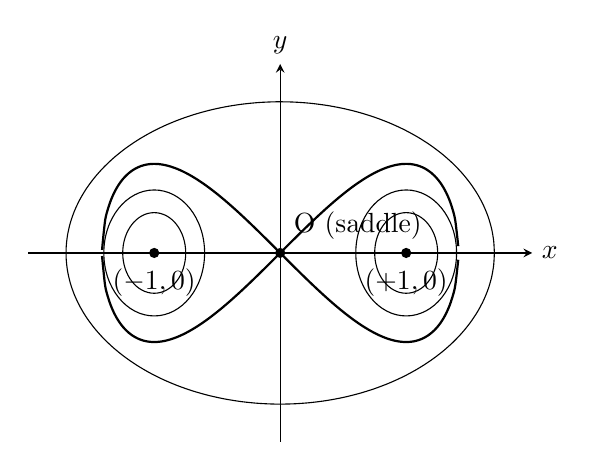
\begin{tikzpicture}[>=stealth, scale=1.6]
  \draw[->] (-2.0,0) -- (2.0,0) node[right] {$x$};
  \draw[->] (0,-1.5) -- (0,1.5) node[above] {$y$};
  % Saddle at origin, separatrix (homoclinic figure-eight): y^2 = x^2 - x^4/2, i.e. H=0
  \draw[thick,domain=-1.414:1.414,smooth,variable=\t,samples=120]
    plot ({\t},{ sqrt(max(0,\t*\t - 0.5*\t*\t*\t*\t)) });
  \draw[thick,domain=-1.414:1.414,smooth,variable=\t,samples=120]
    plot ({\t},{-sqrt(max(0,\t*\t - 0.5*\t*\t*\t*\t)) });
  % Closed orbits inside each well (small)
  \draw (-1,0) ellipse (0.25 and 0.32);
  \draw ( 1,0) ellipse (0.25 and 0.32);
  \draw (-1,0) ellipse (0.4 and 0.5);
  \draw ( 1,0) ellipse (0.4 and 0.5);
  % Outer orbit
  \draw[domain=0:360,smooth,variable=\t,samples=80]
    plot ({1.7*cos(\t)},{1.2*sin(\t)});
  % Markers
  \node[circle,fill,inner sep=1.3pt,label=above right:{O (saddle)}] at (0,0) {};
  \node[circle,fill,inner sep=1.3pt,label=below:{$(-1,0)$}] at (-1,0) {};
  \node[circle,fill,inner sep=1.3pt,label=below:{$(+1,0)$}] at (1,0) {};
\end{tikzpicture}
\end{center}

\subsection*{(c) $a=0$, general $b,c$}

Fixed points require $\dot x=\dot y=0$, so $y^*=0$ and $bx + cx^3 = 0$:
\[ x^*(b + cx^{*2}) = 0. \]
One root is always $x^*=0$. Non-trivial roots require:
\[ cx^{*2} = -b. \]
Solve for $x^*$ when $-b/c>0$:
\[ x^* = \pm\sqrt{-b/c}. \]
Existence condition: $bc<0$.

Jacobian as in (b); characteristic equation $\lambda^2 = -(b+3cx^{*2})$.

\textbf{Origin $(0,0)$:} $\lambda^2=-b$.
\begin{itemize}
\item $b>0$: $\lambda=\pm i\sqrt{b}$ \;$\Rightarrow$\; centre.
\item $b<0$: $\lambda=\pm\sqrt{-b}$ (real, opposite sign) \;$\Rightarrow$\; saddle.
\end{itemize}

\textbf{Side fixed points $x^*=\pm\sqrt{-b/c}$ (require $bc<0$):} substitute $cx^{*2}=-b$ into $b+3cx^{*2}$:
\[ b + 3cx^{*2} = b + 3(-b) = -2b. \]
Eigenvalues:
\[ \lambda^2 = -(b+3cx^{*2}) = 2b. \]
\begin{itemize}
\item $b<0$ ($c>0$): $\lambda^2 = 2b<0$, $\lambda=\pm i\sqrt{-2b}$ \;$\Rightarrow$\; centres.
\item $b>0$ ($c<0$): $\lambda^2 = 2b>0$, $\lambda=\pm\sqrt{2b}$ \;$\Rightarrow$\; saddles.
\end{itemize}

\paragraph{Bifurcation diagram ($x^*$ vs $bc$).} A pitchfork bifurcation at $bc=0$: side branches exist only for $bc<0$.
\begin{center}
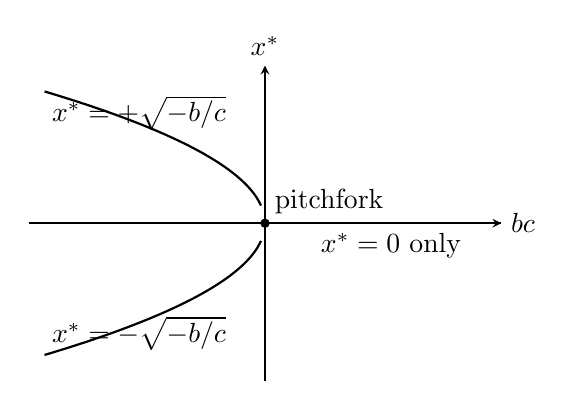
\begin{tikzpicture}[>=stealth, scale=1.0]
  \draw[->] (-3,0) -- (3,0) node[right] {$bc$};
  \draw[->] (0,-2) -- (0,2) node[above] {$x^*$};
  % bc<0 branches (existing): x^* = \pm sqrt(-b/c). Plot as schematic curves.
  \draw[thick,domain=-2.8:-0.05,smooth,variable=\u,samples=60]
    plot ({\u},{ sqrt(-\u) });
  \draw[thick,domain=-2.8:-0.05,smooth,variable=\u,samples=60]
    plot ({\u},{-sqrt(-\u) });
  % bc>=0: only x^*=0 (origin) is shown
  \draw[thick] (-3,0) -- (3,0);
  \node[circle,fill,inner sep=1.2pt] at (0,0) {};
  \node[above right] at (0,0) {pitchfork};
  \node at (-1.6,1.4) {$x^*=+\sqrt{-b/c}$};
  \node at (-1.6,-1.4) {$x^*=-\sqrt{-b/c}$};
  \node[below] at (1.6,0) {$x^*=0$ only};
\end{tikzpicture}
\end{center}
Stability legend: solid branches stable centres for $b<0,c>0$; the central branch is a saddle in that range and a centre for $b>0$.

\paragraph{Phase portrait, $b>0$.} Take $c>0$ first (single well). Origin is a centre, no other fixed points; closed orbits encircle the origin.
\begin{center}
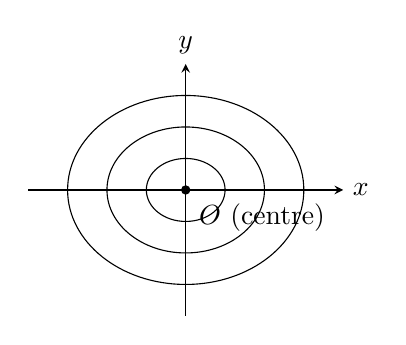
\begin{tikzpicture}[>=stealth, scale=1.0]
  \draw[->] (-2,0) -- (2,0) node[right] {$x$};
  \draw[->] (0,-1.6) -- (0,1.6) node[above] {$y$};
  \draw (0,0) ellipse (0.5 and 0.4);
  \draw (0,0) ellipse (1.0 and 0.8);
  \draw (0,0) ellipse (1.5 and 1.2);
  \node[circle,fill,inner sep=1.2pt,label=below right:{$O$ (centre)}] at (0,0) {};
\end{tikzpicture}
\end{center}
For $b>0,c<0$ (still $b>0$ but inverted quartic): origin is still a centre, and side points $x^*=\pm\sqrt{-b/c}=\pm\sqrt{b/|c|}$ are saddles connected by heteroclinic separatrices that enclose the central centre; orbits inside the separatrix are closed, those outside escape to infinity.

\subsection*{(d) Weak damping, $b<0$, $a^2<4|b|$, fixed points unchanged}

Adding $a>0$ adds $-ay$ to $\dot y$; the Jacobian gains $-a$ on the $(2,2)$ entry:
\[ J = \begin{pmatrix} 0 & 1 \\ -(b+3cx^{*2}) & -a \end{pmatrix}. \]
Compute trace:
\[ \tau = \text{tr}(J) = 0 + (-a) = -a. \]
Compute determinant:
\[ \Delta = \det(J) = (0)(-a) - (1)(-(b+3cx^{*2})) = b + 3cx^{*2}. \]

\begin{itemize}
\item Origin ($b<0,c>0$): $\Delta = b<0$ $\Rightarrow$ saddle (sign of $\Delta$ unchanged).
\item Side wells $x^*=\pm\sqrt{-b/c}$: substitute $cx^{*2}=-b$:
\end{itemize}
Determinant at side wells:
\[ \Delta = b + 3(-b) = -2b = 2|b| > 0. \]
Compute discriminant:
\[ \tau^2 - 4\Delta = a^2 - 8|b|. \]
Use the assumption $a^2 < 4|b|$:
\[ \tau^2 - 4\Delta < 4|b| - 8|b|. \]
Simplify:
\[ \tau^2 - 4\Delta < -4|b| < 0. \]
With $\tau=-a<0$ and $\tau^2-4\Delta<0$, the side wells are \textbf{stable spirals (foci)}.

Modification of the (b) phase portrait: the two centres at $x=\pm 1$ become inward spirals; the saddle at the origin remains, but its homoclinic separatrices break --- trajectories cross between basins only along the unstable manifold of the saddle, otherwise spiral into one well or the other. All orbits eventually reach one of the two stable foci.

\begin{center}
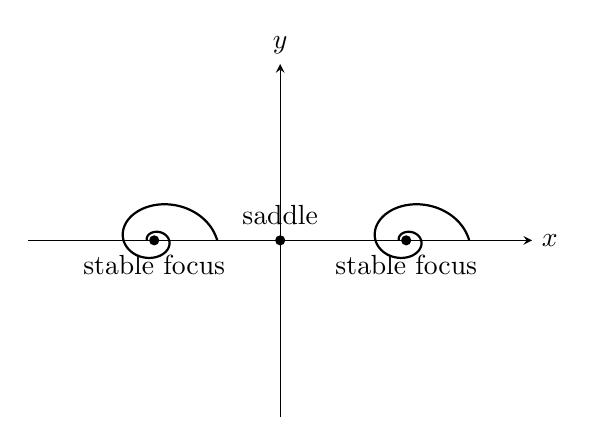
\begin{tikzpicture}[>=stealth, scale=1.6]
  \draw[->] (-2,0) -- (2,0) node[right] {$x$};
  \draw[->] (0,-1.4) -- (0,1.4) node[above] {$y$};
  % Inward spiral around (-1,0)
  \draw[thick,domain=0:540,smooth,variable=\t,samples=160]
    plot ({-1+0.5*exp(-0.004*\t)*cos(\t)},{0.4*exp(-0.004*\t)*sin(\t)});
  \draw[thick,domain=0:540,smooth,variable=\t,samples=160]
    plot ({ 1+0.5*exp(-0.004*\t)*cos(\t)},{0.4*exp(-0.004*\t)*sin(\t)});
  \node[circle,fill,inner sep=1.3pt,label=above:{saddle}] at (0,0) {};
  \node[circle,fill,inner sep=1.3pt,label=below:{stable focus}] at (-1,0) {};
  \node[circle,fill,inner sep=1.3pt,label=below:{stable focus}] at (1,0) {};
\end{tikzpicture}
\end{center}

Physical interpretation: in the double-well potential $V = \tfrac12 b x^2 + \tfrac14 c x^4$ ($b<0$, $c>0$), the unstable equilibrium at the origin separates two stable equilibria. Without damping, the mass oscillates indefinitely about one minimum or the other (or executes large figure-of-eight orbits along the separatrix). With weak drag, energy is dissipated; the mass spirals into whichever well it ends up in --- a bistable mechanical switch.

%==============================================================
\section*{Question 4 --- Freely jointed chain and DNA looping}

\textbf{Problem.} Develop the FJC distribution and its entropic-spring limit; obtain the force--extension relation; apply to DNA-looping probability and the optimum loop size.

\subsection*{(a) 3D distribution}

Independent Gaussian projections multiply:
\[ P(\vb r,N) = P_x(x,N)\,P_y(y,N)\,P_z(z,N). \]
Each factor is $(3/(2\pi Nb^2))^{1/2}\exp(-3x_i^2/(2Nb^2))$, so product of prefactors gives $(3/(2\pi Nb^2))^{3/2}$:
\[ P(\vb r,N) = \!\left(\frac{3}{2\pi N b^2}\right)^{\!3/2}\!\exp\!\left(-\frac{3(x^2+y^2+z^2)}{2 N b^2}\right). \]
Use $r^2 = x^2+y^2+z^2$:
\[ \boxed{\;P(\vb r,N) = \!\left(\frac{3}{2\pi N b^2}\right)^{\!3/2}\!\exp\!\left(-\frac{3 r^2}{2 N b^2}\right).\;} \]
$P_x(x,N)$ is a Gaussian with variance $\sigma_x^2 = Nb^2/3$, so $\sigma_x = b\sqrt{N/3}$. As $N\uparrow$, the distribution flattens and broadens with $\sigma_x\propto\sqrt{N}$.

\paragraph{Sketch of $P_x(x,N)$ for two values of $N$.}
\begin{center}
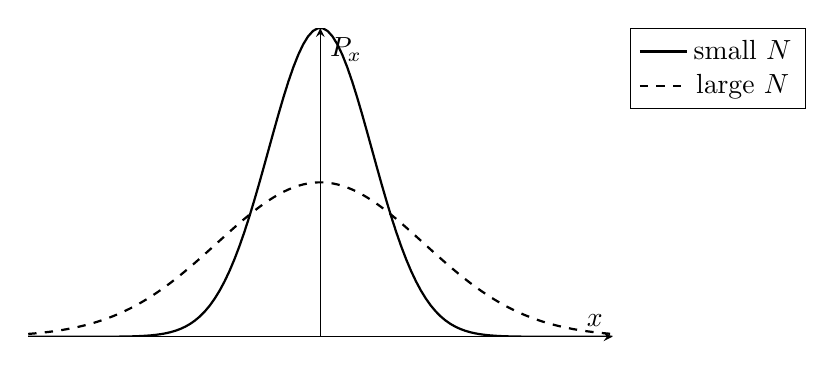
\begin{tikzpicture}[>=stealth, scale=1.0]
  \begin{axis}[axis lines=middle, xlabel=$x$, ylabel=$P_x$,
    width=9cm, height=5.5cm, samples=120, domain=-4:4,
    xtick=\empty, ytick=\empty, legend pos=outer north east]
    \addplot[thick] {1/sqrt(2*pi*0.5)*exp(-x^2/(2*0.5))};
    \addlegendentry{small $N$};
    \addplot[thick,dashed] {1/sqrt(2*pi*2)*exp(-x^2/(2*2))};
    \addlegendentry{large $N$};
  \end{axis}
\end{tikzpicture}
\end{center}

Brownian-motion analogy: the chain end position $\vb r$ after $N$ steps of length $b$ is the sum of independent unit-length random vectors, identical to the position of a random walker after $N$ steps. By the central limit theorem, both produce Gaussian distributions with $\langle r^2\rangle = Nb^2$; the chain configuration is the spatial counterpart of a Brownian trajectory.

\subsection*{(b) Entropic spring}

Boltzmann entropy:
\[ S(\vb r) = k_B \ln P(\vb r,N) + \text{const}. \]
Take the log of the Gaussian:
\[ \ln P = \tfrac32\ln\!\left(\frac{3}{2\pi N b^2}\right) - \frac{3 r^2}{2 N b^2}. \]
Multiply by $k_B$:
\[ S(\vb r) = k_B\,\tfrac32\ln\!\left(\frac{3}{2\pi N b^2}\right) - k_B\,\frac{3 r^2}{2 N b^2}. \]
Helmholtz free energy at fixed $T$, with $U=0$ for an FJC:
\[ F(\vb r) = U - T S(\vb r) = -T S(\vb r). \]
Substitute $S$:
\[ F(\vb r) = -\tfrac32 k_B T\ln\!\left(\frac{3}{2\pi N b^2}\right) + \frac{3 k_B T}{2 N b^2}\,r^2. \]
Identify the form $F = d + cr^2$ with $d=-\tfrac32 k_BT\ln(3/(2\pi Nb^2))$:
\[ \boxed{\;F(\vb r) = d + c\,r^2,\qquad c = \frac{3 k_B T}{2 N b^2},\qquad d=\text{const}(T,N).\;} \]
$F$ is quadratic in $r$, so $-\nabla F = -2c\vb r$ acts as a Hooke restoring force with stiffness $\kappa = 2c = 3 k_B T/(N b^2)$. The chain has no internal energy --- its restoring force comes entirely from loss of conformational entropy when extended (an entropic spring).

Temperature dependence: $\kappa\propto T$. The entropic stiffness grows linearly with temperature.

\subsection*{(c) Force--extension under tension $f$}

Single segment $\vb b_i$ with $|\vb b_i|=b$ has energy $-fb\cos\theta_i$ when $\vb f = f\hat{\vb z}$ acts on the chain end. Single-segment partition function (integrate over orientation):
\[ Z_1 = \int_0^{2\pi}\!\de\phi\!\int_0^{\pi}\!e^{f b\cos\theta/(k_BT)}\sin\theta\,\de\theta. \]
Perform the $\phi$ integral:
\[ Z_1 = 2\pi\!\int_0^{\pi}\!e^{a\cos\theta}\sin\theta\,\de\theta,\qquad a=\frac{fb}{k_BT}. \]
Substitute $u=\cos\theta$, $\de u=-\sin\theta\,\de\theta$:
\[ Z_1 = 2\pi\!\int_{-1}^{1} e^{a u}\,\de u. \]
Evaluate the integral:
\[ Z_1 = 2\pi\,\frac{e^a - e^{-a}}{a}. \]
Recognise $\sinh a = (e^a-e^{-a})/2$:
\[ Z_1 = \frac{4\pi\sinh a}{a}. \]
Independent segments multiply:
\[ Z = Z_1^{N} = \!\left(\frac{4\pi\sinh a}{a}\right)^{\!N}. \]
Take the log:
\[ \ln Z = N\!\left[\ln(4\pi) + \ln\sinh a - \ln a\right]. \]
Mean extension along $\vb f$ from $\langle z\rangle = k_B T\,\partial\ln Z/\partial f$:
\[ \langle z\rangle = k_BT\,\pd{\ln Z}{f}. \]
Use chain rule with $\partial a/\partial f = b/(k_BT)$:
\[ \langle z\rangle = k_B T\cdot\frac{b}{k_BT}\,N\,\pd{}{a}(\ln\sinh a - \ln a). \]
Differentiate term by term:
\[ \pd{}{a}(\ln\sinh a - \ln a) = \coth a - \frac{1}{a}. \]
Hence
\[ \boxed{\;\langle z\rangle = N b\!\left(\coth a - \frac{1}{a}\right)\equiv N b\,\mathcal L(a),\qquad a=\frac{fb}{k_B T}.\;} \]

Low-force limit $a\ll 1$: use $\coth a\approx a/3 + 1/a$:
\[ \coth a - \frac{1}{a} \approx \frac{a}{3}. \]
Substitute into the boxed result:
\[ \langle z\rangle \approx N b\,\frac{a}{3}. \]
Substitute $a = fb/(k_BT)$:
\[ \langle z\rangle \approx \frac{N b^2 f}{3 k_B T}. \]
Solve for $f$:
\[ \boxed{\;f \approx \frac{3 k_B T}{N b^2}\langle z\rangle.\;} \]
A linear (Hookean) force--extension with the same stiffness $\kappa = 3 k_B T/(N b^2)$ as in (b).

\subsection*{(d) DNA looping probability}

Treat dsDNA as a FJC with statistical (Kuhn) segment $b = 2P$. Convert $P=150$ bp to nm using $\SI{0.34}{nm/bp}$:
\[ P = 150\times 0.34\,\text{nm} = \SI{51}{nm}. \]
Kuhn length:
\[ b = 2P = \SI{102}{nm}. \]
For a chain of contour length $\lambda$:
\[ N = \frac{\lambda}{b}. \]
Probability that the two ends coincide ($\vb r = 0$, evaluated as the value of the Gaussian density at the origin):
\[ p(\lambda) = P(\vb r=0,N) = \!\left(\frac{3}{2\pi N b^2}\right)^{\!3/2}. \]
Strip prefactors to display $N$-dependence:
\[ \boxed{\;p(\lambda) \propto N^{-3/2}.\;} \]
Entropy difference between the looped state and a free chain:
\[ \Delta S = k_B \ln p(\lambda). \]
Take the log of the Gaussian prefactor:
\[ \Delta S = k_B\!\left[\tfrac32\ln\!\left(\frac{3}{2\pi b^2}\right) - \tfrac32\ln N\right]. \]
Collect constants into $C$:
\[ \boxed{\;\Delta S = k_B\!\left(C - \tfrac32 \ln N\right).\;} \]

\subsection*{(e) Optimum loop size}

Loop free energy = elastic bending + entropic cost:
\[ \Delta G_\text{loop} = \Delta G_\text{bend} - T\,\Delta S. \]
Insert the given bending energy:
\[ \Delta G_\text{loop} = \frac{\pi P}{R} k_B T - T\,\Delta S. \]
For a loop of contour length $\lambda$ closing into a circle of radius $R$, $2\pi R = \lambda$:
\[ R = \frac{\lambda}{2\pi}. \]
Substitute $R$ into the bending term:
\[ \frac{\pi P}{R}k_B T = \frac{2\pi^2 P}{\lambda}k_B T. \]
Substitute $\Delta S = k_B(C - \tfrac32\ln N)$:
\[ -T\,\Delta S = \tfrac32 k_B T\,\ln N - C\,k_B T. \]
Combine the two contributions:
\[ \boxed{\;\Delta G_\text{loop}(\lambda) = \frac{2\pi^2 P}{\lambda}k_B T + \tfrac32 k_B T\,\ln N - C\,k_B T,\qquad N = \lambda/b.\;} \]

Behaviour: at small $\lambda$, the elastic $1/\lambda$ term dominates --- bending is prohibitive. At large $\lambda$, the $\tfrac32\ln N$ term dominates --- entropic cost of bringing distant ends together. There is a minimum at intermediate length.

\paragraph{Sketch.}
\begin{center}
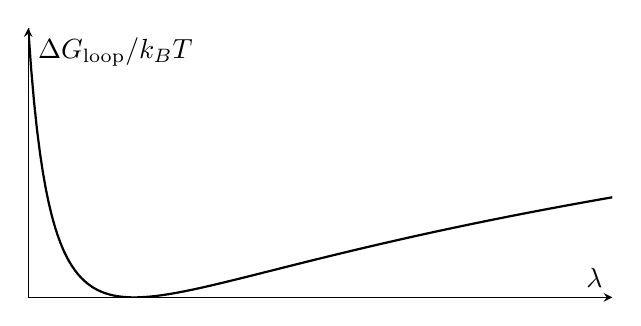
\begin{tikzpicture}[>=stealth, scale=1.0]
  \begin{axis}[axis lines=middle, xlabel=$\lambda$, ylabel=$\Delta G_\text{loop}/k_B T$,
    width=9cm, height=5cm, samples=200, domain=0.3:6,
    xtick=\empty, ytick=\empty]
    \addplot[thick] {2/x + 1.5*ln(x) + 1};
  \end{axis}
\end{tikzpicture}
\end{center}

Minimise: note $\partial\ln N/\partial\lambda = \partial\ln(\lambda/b)/\partial\lambda = 1/\lambda$. Differentiate:
\[ \dv{\Delta G_\text{loop}}{\lambda} = -\frac{2\pi^2 P}{\lambda^2}k_B T + \frac{3 k_B T}{2\lambda}. \]
Set to zero:
\[ -\frac{2\pi^2 P}{\lambda^2}k_B T + \frac{3 k_B T}{2\lambda} = 0. \]
Multiply by $\lambda^2/(k_BT)$:
\[ -2\pi^2 P + \tfrac32 \lambda = 0. \]
Solve for $\lambda$:
\[ \lambda_\text{min} = \frac{4\pi^2 P}{3}. \]
Numerical with $P=\SI{51}{nm}$:
\[ \lambda_\text{min} = \frac{4\pi^2}{3}\times 51\,\text{nm}. \]
Evaluate the prefactor:
\[ \frac{4\pi^2}{3} \approx 13.16. \]
Multiply:
\[ \lambda_\text{min} \approx 13.16 \times 51\,\text{nm} \approx \SI{671}{nm}. \]
Convert to bp using $0.34\,\text{nm/bp}$:
\[ \lambda_\text{min}/\text{bp} \approx 671/0.34 \approx 1970. \]
\[ \boxed{\;\lambda_\text{min} \approx \SI{670}{nm} \approx 2000\,\text{bp}.\;} \]

\end{document}
